\documentclass[fleqn,varvw,preprintnumbers,citeautoscript]{memo}

\usepackage[utf8]{inputenc}
\usepackage[T1]{fontenc}

\graphicspath{{../../fig/}}
\usepackage[caption=false]{subfig}
\usepackage{enumerate}


\newcommand\vlong{V_\text{long}}

\begin{document}

\title{Memo 2: definizione degli strumenti necessari per la misura}

\author{Francesco Polleri}
\email{s5025011@studenti.unige.it}
\author{Mattia Sotgia}
\email{s4942225@studenti.unige.it}

\collaboration{Gruppo A1}
\affiliation{Dipartimento di Fisica, Università degli Studi di Genova, I-16146 Genova, Italia}

\author{Lorenzo Lucentini}
\author{Michele Giorgi}
\collaboration{Gruppo C6}
\affiliation{Dipartimento di Fisica, Università degli Studi di Genova, I-16146 Genova, Italia}

\revised{\today}
\preprint{MEMO/2 (\today)}

\begin{abstract}

\end{abstract}
\maketitle

\section{Progettazione del circuito}

Il circuito complessivo (a meno dell'elettromagnete che vediamo in un successivo memo) consta di quattro principali elementi che vogliamo progettare e poi caratterizzare in base alle necessità che ci siamo imposti nel memo 1 per l'esperimento che vogliamo realizzare: \begin{enumerate}[1.]
    \item Generatore di corrente per l'alimentazione della sonda;
    \item Amplificatore operazionale per strumentazione;
    \item Sonda con resistenze da \SI{500}{\ohm} di protezione;
    \item Sistema di controllo e presa dati (Arduino DUE/Mega 256);
\end{enumerate}

Troviamo uno schema complessivo con anche riportati i valori di progettazione in figura \ref{fig:circuit_memo2}.

\subsection{Progettazione del generatore di corrente}

Il generatore di corrente vogliamo che fornisca in uscita una corrente $i=\SI{10}{\milli\ampere}$, dato in ingresso una differenza di potenziale ai capi $V^+$ e $V^-$ pari a $\Delta V = [\SI{1}{\volt}, \SI{10}{\volt}]$. Abbiamo che \begin{equation}
    i_\text{out} = \frac{R_2}{R_1}\frac{V^--V^+}{R_5}\label{eq:gen}
\end{equation} dove \[\frac{R_1}{R_2} = \frac{R_3}{R_4}=k.\]

Vogliamo ottenere una corrente in uscita di circa \SI{10}{\milli\ampere}, quindi possiamo scegliere $R_1=R_2=R_3=R_4=\SI{1}{\kilo\ohm}$, per fare si che il coefficiente $R_2/R_1$ di (\ref{eq:gen}) si possa semplificare a 1. La scelta di $R_5$ è quindi l'unica che dobbiamo effettuare per dover scegliere poi il valore di $\Delta V$ e ottenere il valore di $i$.

\subsection{Progettazione dell'amplificatore di tensione per strumentazione}

L'amplificatore per strumentazione serve per amplificare la tensione di Hall che misuriamo ai capi della sonda, vogliamo ottenere un guadagno di circa 200, quindi sfruttando la divisione in due stadi dell'amplificatore possiamo ottenere una prima fase con guadagno di circa 20 e una seconda fase con un guadagno di circa 10. Il guadagno differenziale di un amplificatore per strumentazione possiamo ottenerlo come (posti $R_b'=R_b$, $R_c'=R_c$ e $R_d=R_d'$)\begin{equation}
    G= \frac{R_d}{R_c}\qty(1+2\frac{R_b}{R_a}).\label{eq:gain_diff}
\end{equation} Utilizziamo allora resistenze di valori $R_a=R_c=R_c'=\SI{1}{\kilo\ohm}$ e $R_b=R_b'=R_d=R_d'=\SI{10}{\kilo\ohm}$.

\section{Correzione degli errori di misura di $V_H$}

\paragraph{Offset} Facendo un primo test della strumentazione osserveremmo un offset della tensione in uscita dall'amplificatore legata al suo funzionamento. Quindi la relazione \begin{equation}
    V_\text{read} = GV_H = G\frac{i}{wen}B
\end{equation} diventa \begin{equation}
    V_\text{read} = GV_H + V_\text{offset} = G\frac{i}{wen}B + V_\text{offset}\label{eq:offset},
\end{equation} che possiamo correggere nel fit dei dati sperimentali e ottenere quindi un valore di offset. 

\paragraph{Effetto longitudinale $V_\text{long}$} Se la sonda è leggermente imprecisa nella costruzione, ovvero se i punti dove misuriamo $V_H$ non sono precisamente ortogonali alla direzione di $\va{J}$ e della corrente, osserviamo che il campo elettrico che misuriamo attraverso $V_H$ è in realtà diverso da zero in assenza di un campo magnetico $B$, infatti avremo una lettura della corrente che attraversa il circuito. Però osserveremmo che questo contributo si comporta come $B^2$, quindi che non interessa effettivamente la nostra misura in maniera influente. Infatti, eseguendo un fit come \begin{equation}
    V_\text{read} = kB^2 +  GV_H + V_\text{offset} = kB^2 + G\frac{i}{wen}B + V_\text{offset},\label{eq:B2_dep}
\end{equation} osserviamo che il valore di $k\neq0$, quindi possiamo togliere anche il contributo legato al termine quadratico. 

\subsection{Possibile quantificazione dell'effetto di $V_\text{offset}$ e $V_\text{long}$}

 Rispetto a quanto abbiamo detto sugli effetti che possiamo osservare sulla tensione in uscita considerando $i=0$, possiamo per ogni punto della presa dati anche quantificare il valore di $V_\text{offset}$ e il valore di $V_\text{long}$. 

Infatti, imponendo la corrente $i$ nulla possiamo effettivamente trovare il valore di offset della tensione in uscita dall'amplificatore. In questo modo possiamo quindi ottenere un valore di offset quantitativo reale da confrontare con il valore che otteniamo dal fit di (\ref{eq:offset}). 

Vorremmo provare anche definire l'effetto di $\vlong$ e quindi anche trovare un modo per correggerlo, e rimuoverlo dalla misura. La causa di $\vlong$ è da ricercarsi in un difetto di costruzione della sonda che però si presenta in modo asimmetrico (fig. \ref{fig:sonda_schema}). Poichè il problema però appare non simmetrico, allora possiamo ipotizzare che se riuscissimo a invertire il verso del campo elettrico $\va{E}_H$ che si viene a formare potremmo allora ottenere in qualche modo di isolare il contributo quadratico in $B$. 

La tensione di Hall viene misurata come differenza tra i capi $+V_H$ e $-V_H$, che come vediamo nello schema di fig. \ref{fig:sonda_schema} risultano essere disallineati di un certo $\delta$. 

\begin{figure}
    \centering
    \subfloat[][]{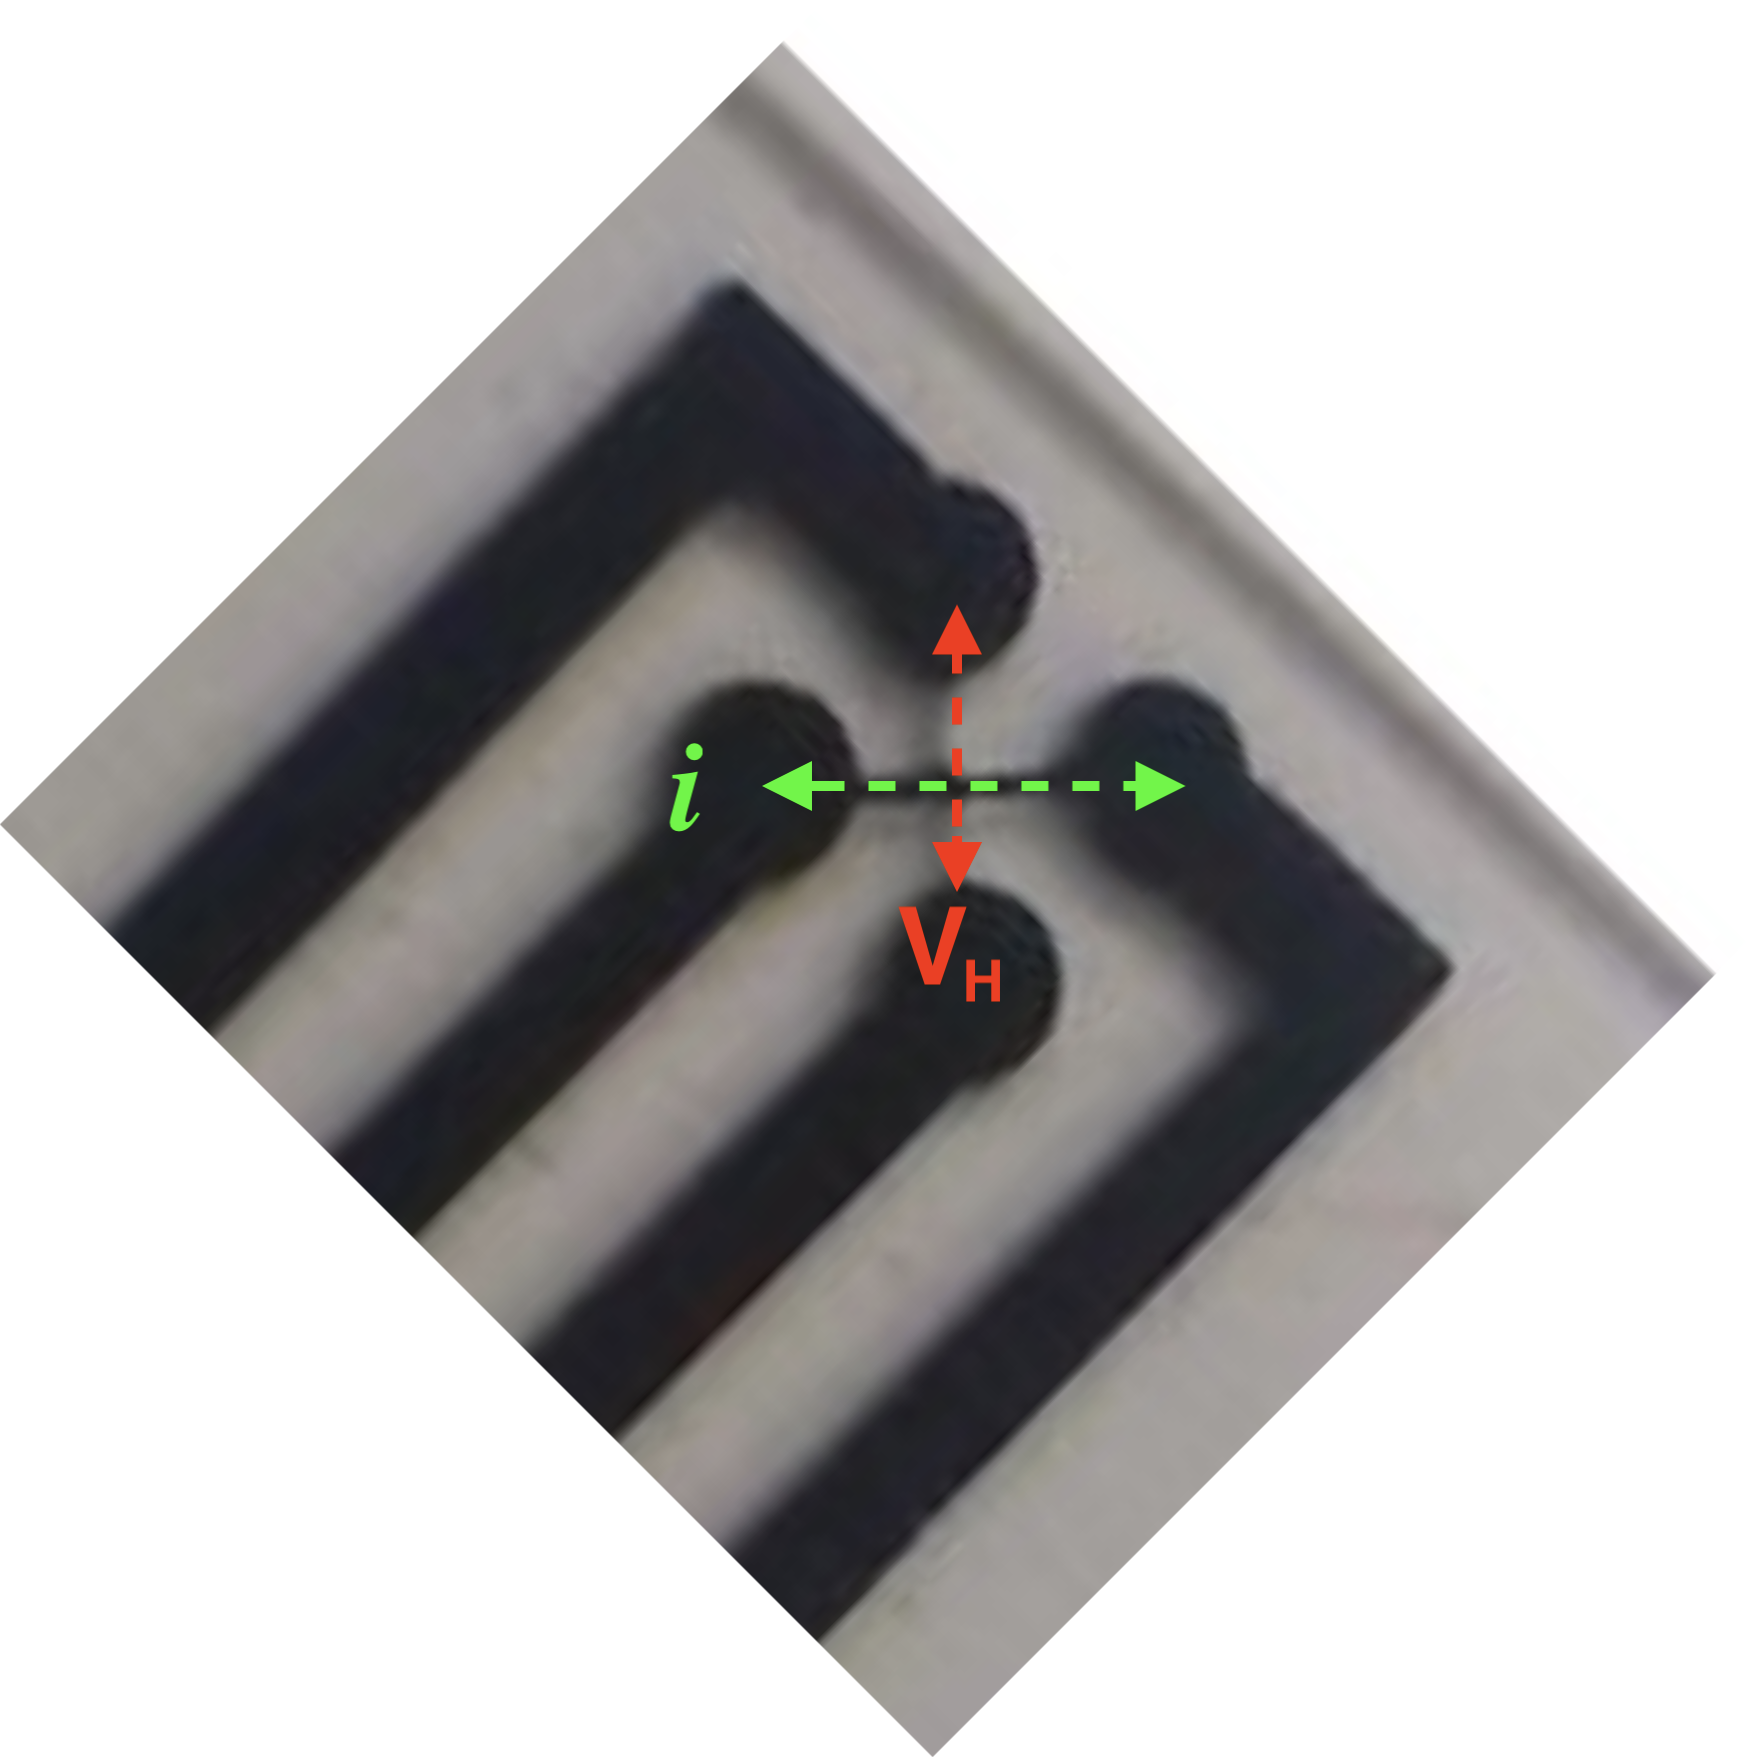
\includegraphics[width=0.25\linewidth]{zoomed_sonda.png}\label{fig:sonda_img}}\hspace{1cm}
    \subfloat[][]{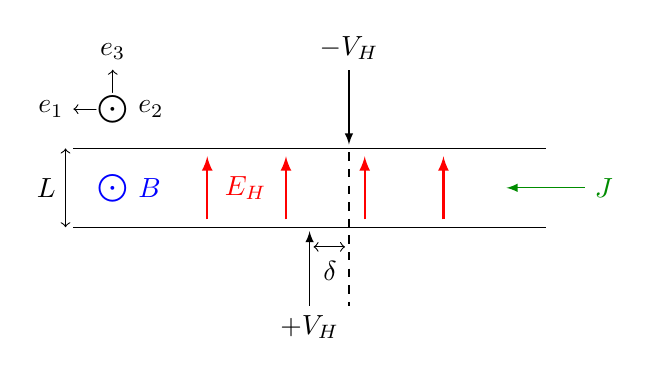
\begin{tikzpicture}
    \draw[<->] (0,1.5) node[left] {$\vu{e}_1$} -| (0.5,2) node[above] {$\vu{e}_3$};
    \draw (0.7,1.5) node[right] {$\vu{e}_2$};
    \filldraw[white] (0.5, 1.5) circle (0.2) node[black] {$\mathbf{\bigodot}$};
    \draw (0,0) -- (6,0) (0,1) -- (6,1);
    \draw[latex-, black!45!green] (5.5, 0.5) to (6.5,0.5) node[right] {$\va{J}$};
    \foreach \i in {1,...,4} \draw[-latex,thick, red] (\i+0.7,0.1) to (\i+0.7,0.9)
    ;
    \draw[red] (1.8,0.5) node[right] {$\va{E}_H$};
    \filldraw[white] (0.5, 0.5) circle (0.2) node[blue] {$\mathbf{\bigodot}$};
    \draw[blue] (0.7,0.5) node[right] {$\va{B}$};
    \draw[latex-] (3,-0.05) to (3, -1) node[below]{$+V_H$};
    \draw[latex-] (3.5,1.05) to (3.5, 2) node[above]{$-V_H$};
    \draw[dashed] (3.5,0.95) to (3.5,-1);
    \draw (3.05, -0.55) node[right] {$\delta$};
    \draw[<->] (3.05, -1+0.75) to (3.45,-1+0.75);
    \draw[<->] (-0.1,0) to (-0.1,1);
    \draw (-0.1,0.5) node[left] {$L$}
    ;
\end{tikzpicture}\label{fig:sonda_schema}}
    \caption{(a) Ingrandimento ruotato di \SI{45}{\deg} della sonda. (b) Rappresentazione del problema relativo all'effetto della misura di $\vlong$.}
\end{figure}

Nel caso ideale (ovvero sistema simmetrico) abbiamo che la tensione tra i due capi $+$ e $-$ può essere misurata come \begin{equation}
    V_H = \frac{i}{wen}B. 
\end{equation} 

Quando però invertiamo la polarizzazione del campo magnetico, ovvero invece che considerarlo uscente come $\va{B} = B\vu{e}_2$ lo consideriamo entrante come $\va{B} = -B\vu{e}_2$, allora possiamo ottenere che, dalla forza di Lorentz, lasciando la corrente scorrere nella stessa direzione (per cui ho $\va{J} = J\vu{e}_1$), l'effetto dovrebbe risultare in un campo elettrico diretto come $\va{E} = -E_H \vu{e}_3$, opposto all'effetto che otterremo nel caso precedente. 

Il termine quadratico in $B$ è introdotto da un difetto che come abbiamo detto non è simmetrico rispetto al verso della corrente (o, per analogie, al verso del campo magnetico). Invertendo quindi il campo magnetico dovremmo osservare che il termine in $B^2$ non dovrebbe cambiare. Consideriamo quindi i due casi \begin{enumerate}[1.]
    \item se $B=B^+>0$ (ovvero se siamo nel caso per cui $\va{B} = B\vu{e}_2$), allora abbiamo che la differenza di tensione che leggiamo ai capi $+V_H$ e $-V_H$ risulterà essere (tenendo conto di tutti i termini di correzione introdotti in (\ref{eq:B2_dep}) e dell'amplificazione del circuito) \begin{equation}
        V_H^+ = kB^2 + G\frac{i}{wen}B^+ + V_\text{offset};\label{eq:VH+}
    \end{equation}
    \item se invece consideriamo $B=B^-<0$ (ovvero se siamo nel caso per cui $\va{B} = -B\vu{e}_2$) allora avremo che la differenza tensione letta, se consideriamo $B^- = -B^+$ \begin{equation}
        V_H^- = kB^2 - G\frac{i}{wen}B^+ + V_\text{offset}.\label{eq:VH-}
    \end{equation}
\end{enumerate}
Confrontando la (\ref{eq:VH+}) e la (\ref{eq:VH-}) otteniamo che (nell'ipotesi che le due tensioni di offset siano uguali\footnote{Non troviamo un valido motivo per cui le due tensioni di offset non dovrebbero esserlo, non dipendendo teoricamente in alcun modo dal campo magnetico a cui è sottoposta la sonda.}) la differenza \begin{equation}
    V_H^+ - V_H^- = 2\frac{GiB^+}{wen}
\end{equation} ci permette di ottenere una misura di $V_H$ effettivamente libera dal termine in $B^2$, con anche l'aggiunto beneficio di cancellare anche l'effetto di un offset sulla tensione (se si verificano le ipotesi di cui abbiamo detto sopra), al costo di dover effettuare per ogni campo magnetico $B$ anche una misura con il rispettivo campo magnetico $-B$, di uguale intensità ma direzione opposta\footnote{Questo non risulta essere poi tanto un problema se possiamo trovare il modo di inserire la misura doppia con $B$ e con $-B$ automatizzando il processo di presa dati.}. Inoltre in questo modo possiamo anche ottenere che \begin{equation}
    V_H^++V_H^- = 2\qty(V_\text{offset} + k\qty(B^+)^2),
\end{equation} ovvero possiamo anche quantificare il valore di $k$ tramite misura diretta (noto $V_\text{offset}$).

\begin{turnpage}
    \begin{figure*}[p]
        \centering
        % 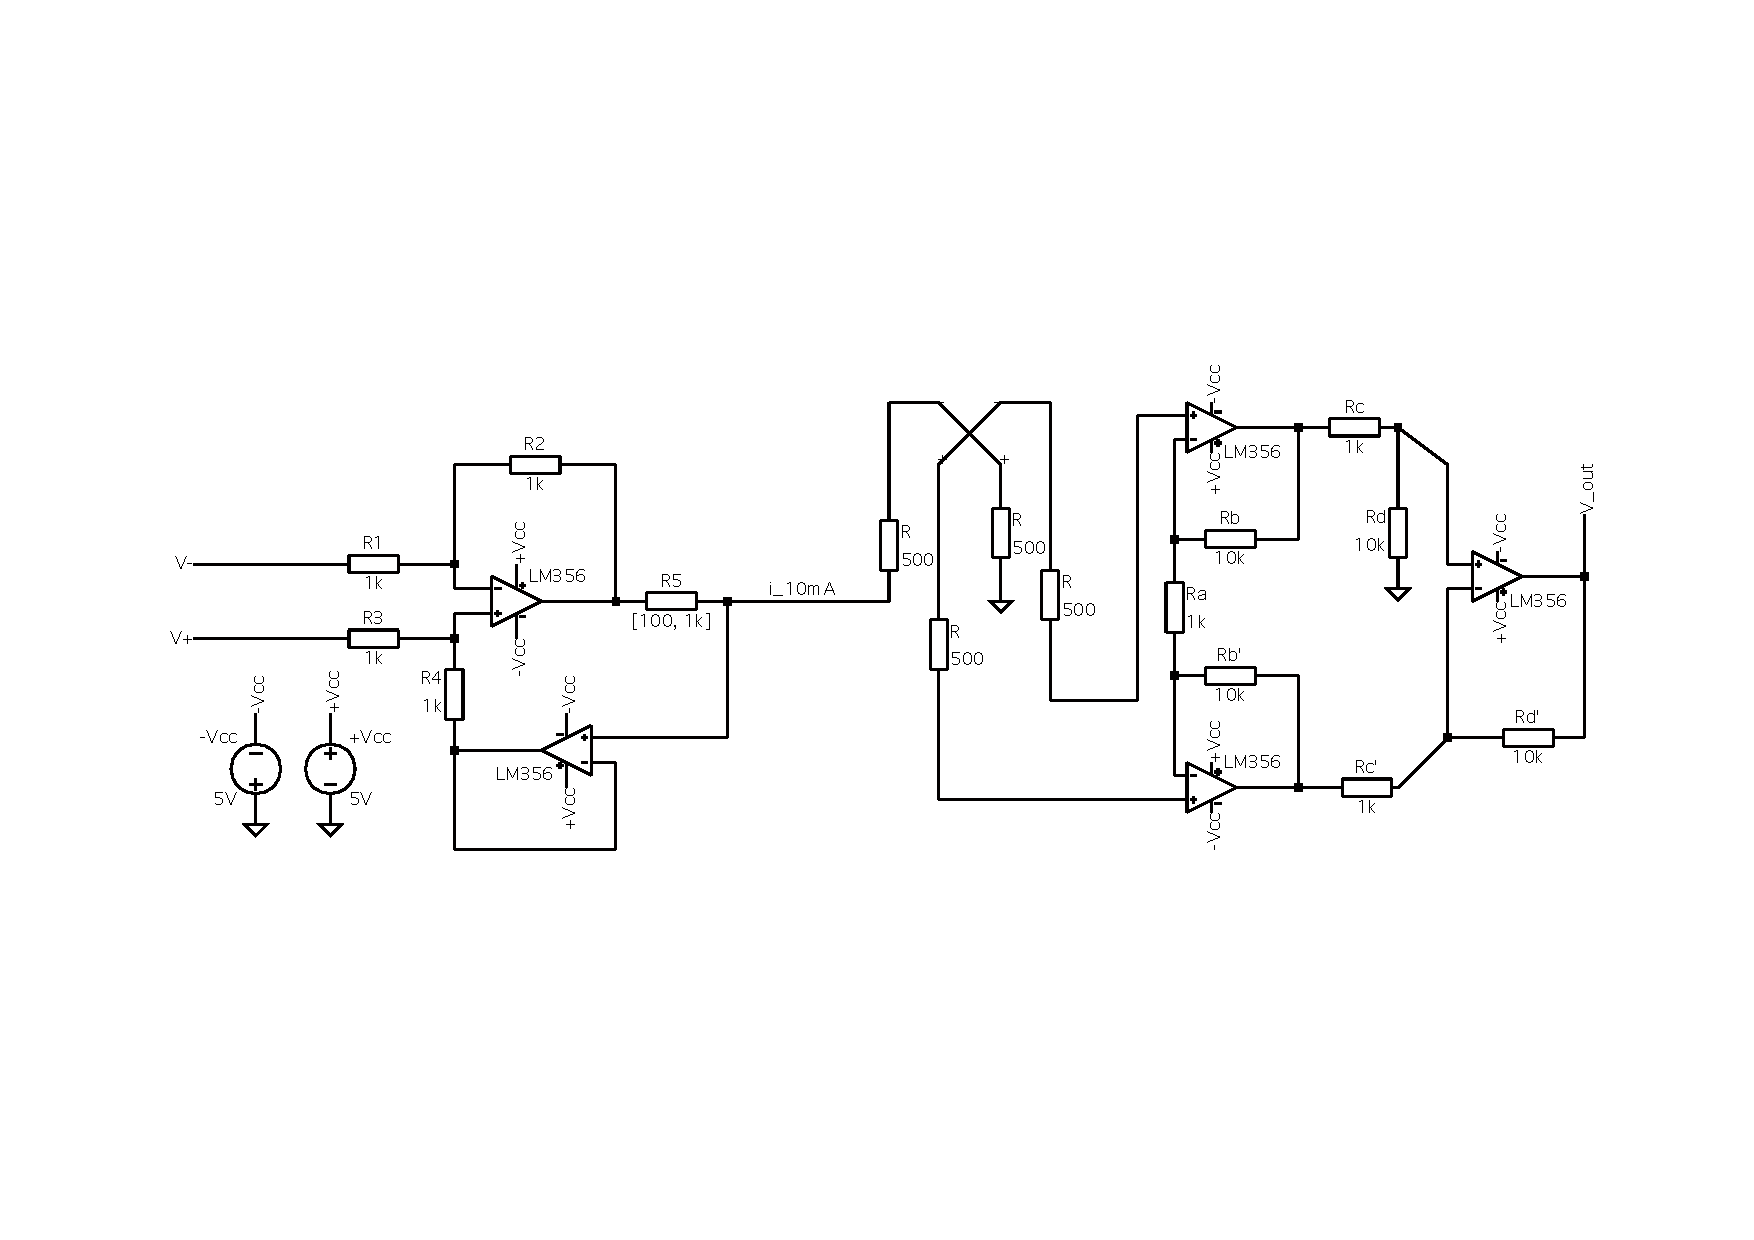
\includegraphics[width=\linewidth,trim={2cm 6.5cm 2cm 6cm},clip]{memo2_full_circuit.pdf}
        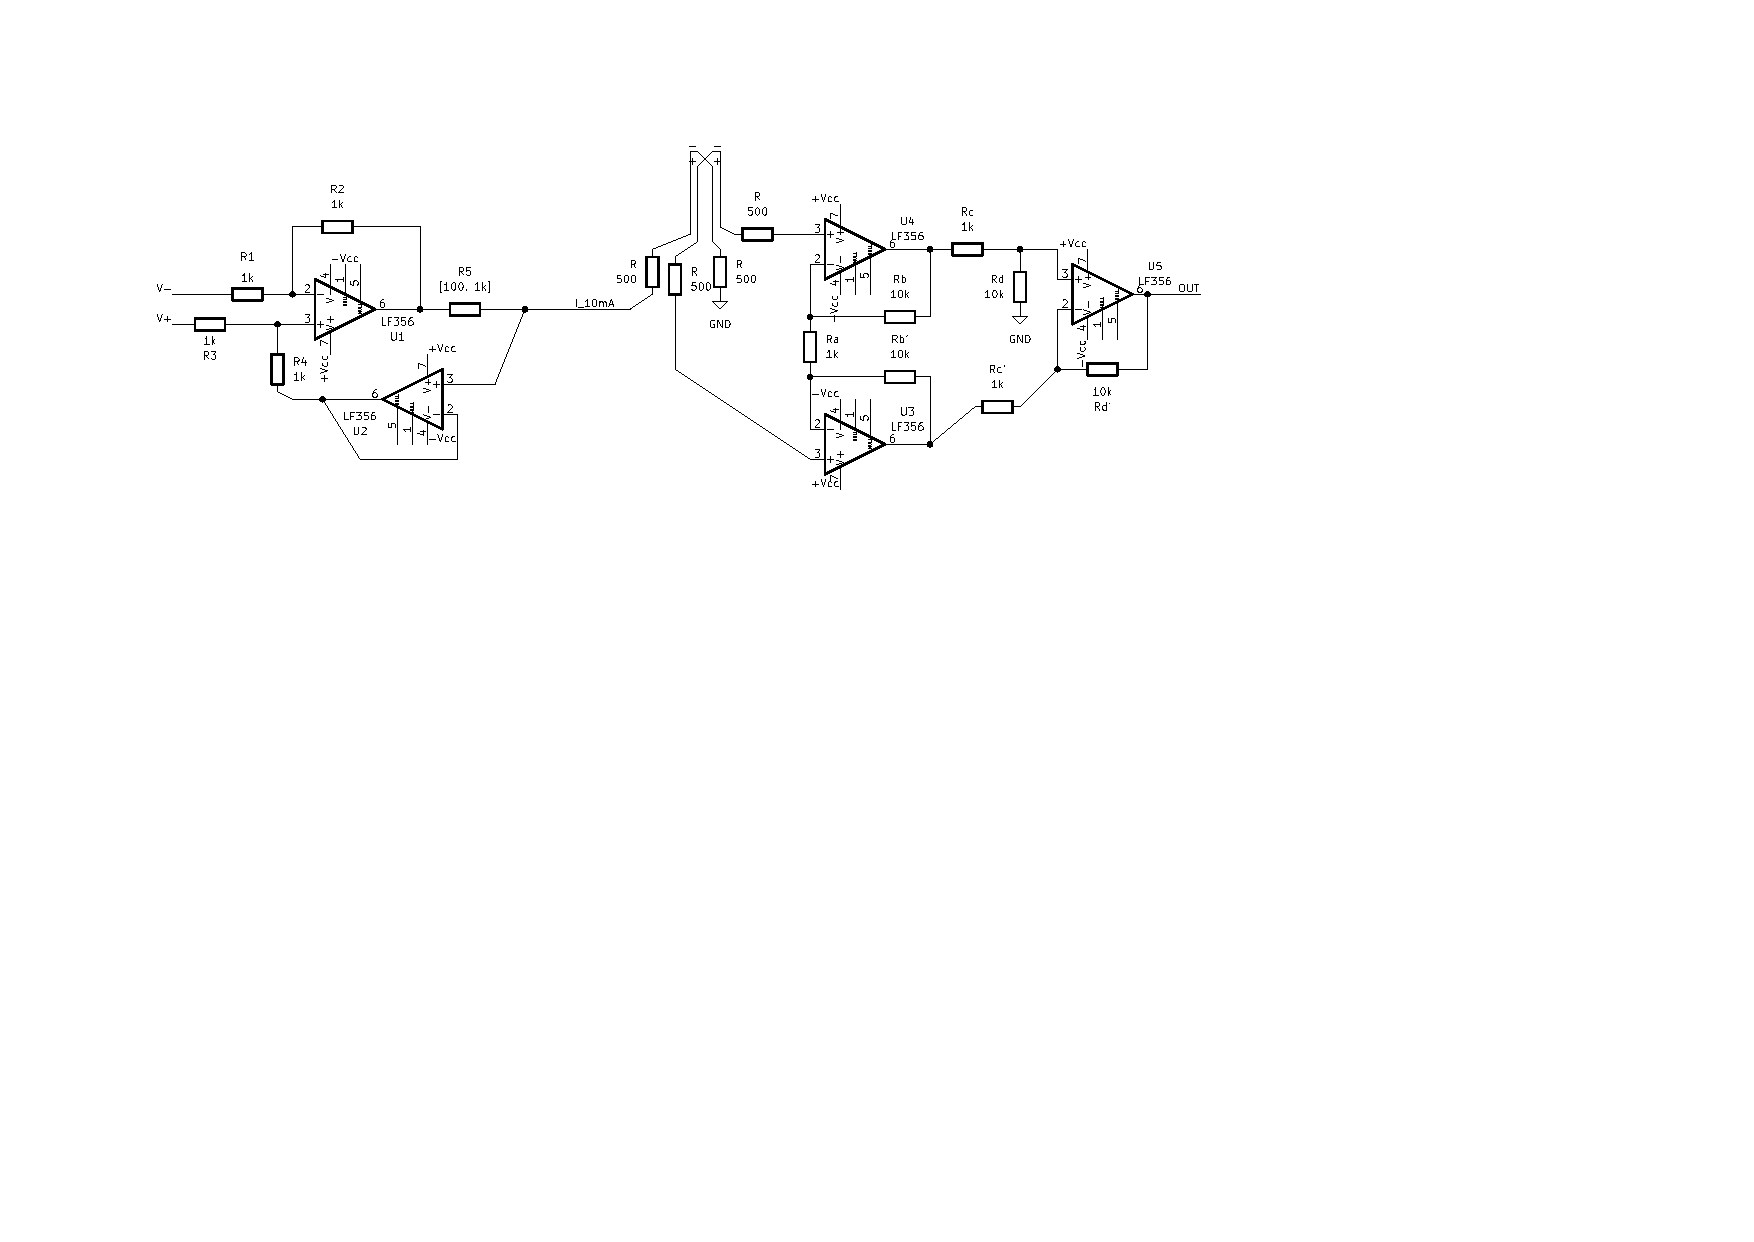
\includegraphics[width=\linewidth,trim={2.5cm 12.5cm 8cm 2cm},clip]{SCHEMA_full1.pdf}
        \caption{Circuito completo delle tre componenti principali (da sinistra a destra sono inseriti il generatore di corrente, la sonda e l'amplificatore differenziale per strumentazione).}\label{fig:circuit_memo2}
    \end{figure*}
\end{turnpage}

\end{document}